\section{Feedforward Neural Networks}
\label{sec:feedforward_neural_networks}
A natural extension of the perceptron model is to combine multiple perceptrons in a network architecture called a neural network. It is intuitively clear that, much like in an organic brain, a complex arrangement of many simple computing units can learn much more complicated functions than those simple units alone. In this section, we will examine how such a network architecture based on perceptrons can be constructed. The ideas that we develop are mostly based on Ref. \cite[Ch.\,6]{DBLP:books/daglib/0040158}.

\subsection{Extensions to the Perceptron}
Before explaining the composition of perceptrons to neural networks, we will first explore two common extensions to the perceptron model which are required in the network architecture we develop.

First, we introduce an additional term called \emph{bias} to the output calculation. The new output $\hat{y}$ becomes
\begin{equation}\label{eq:perceptron2}
\hat{y} = \sign(\bm{w}^\top\bm{x} + b),
\end{equation}
where the scalar $b$ is the bias. This additional learnable parameter shifts the function computed by the model \emph{independently of its input}. Learning a bias value can therefore help the model make better predictions.

Second, we generalize the perceptron by replacing the $\sign$ function with an arbitrary function $f$ called \emph{activation function}. In contrast to $\sign(x)$, most activation functions used in neural networks are continuous, since this enables us to use a variety of \emph{gradient-based} learning algorithms for training as we will see in Section \ref{sec:training}. Concrete examples of activation functions will be discussed later in this section.

We also introduce the quantity $z$, the \emph{weighted input}, which simply is defined as
\begin{equation}\label{eq:perceptron3}
z = \bm{w}^\top\bm{x} + b.
\end{equation}

The computing units we have obtained with these modifications to the perceptron are generally called \emph{neurons} or simply \emph{units}.

\subsection{Network architecture}
Any arrangement of neurons in a network architecture can be considered a neural network. The most influential such architecture is the feedforward neural network, which forms the basis for many other more advanced neural networks \cite[Ch.\,6,\,p.\,163]{DBLP:books/daglib/0040158}. Feedforward neural networks are sometimes also called \emph{multilayer perceptrons} (MLPs).

In feedforward neural networks, the computing units are arranged in layers. We distinguish between the \emph{output layer}, the \emph{hidden layers}, and the \emph{input layer}. The output layer is the final layer in the network were its actual output is produced. The input layer is the first layer in the network, and all layers in between are called hidden layers. The input layer is special in that it does not compute anything; it merely represents the input that is passed into the neural network. In general, a $L$-layer feedforward neural network consists of one input layer, $(L-2)$ hidden layers, and an output layer. We call the number of layers $L$ the \emph{depth} of the model.

Every neuron in a layer $l$ receives input from all neurons in the \nth{(l-1)} layer. There are no connections between neurons in the same layer, and we also do not allow feedback connections into previous layers. Neurons in the hidden and output layers behave exactly like the modified perceptron; the only important detail is that their input is the output from the previous layer. An illustration of a feedforward neural network can be found in Fig. \ref{fig:network}.
\begin{figure}
	\begin{center}
		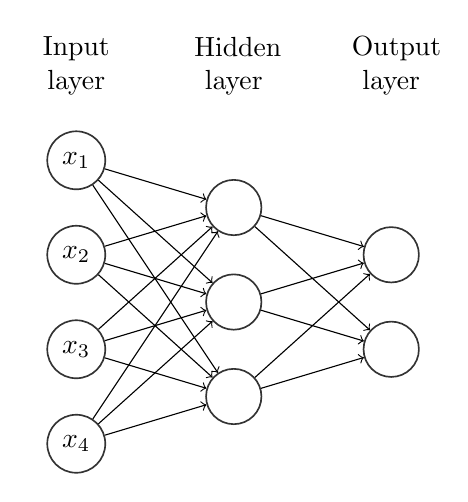
\begin{tikzpicture}
	\tikzstyle{neuron} = [circle,draw=black!80,semithick,minimum size=20pt]
	\tikzstyle{layer} = [text width=1cm, align=center]
	% input layer
	\node[layer] at (0, 0) {Input layer};
	\foreach \i in {1,...,4}
		\node[neuron] (input\i) at (0, -\i*1.2) {$x_\i$};
	% hidden layer
	\node[layer] at (2, 0) {Hidden layer};
	\foreach \i in {1,...,3}
		\node[neuron] (hidden\i) at (2, -\i*1.2 -.6) {};
	% output layer
	\node[layer] at (4, 0) {Output layer};
	\foreach \i in {1,...,2}
		\node[neuron] (output\i) at (4, -\i*1.2 -1.2) {};
	% connections input->hidden
	\foreach \i in {1,...,4}
		\foreach \j in {1,...,3}
			\draw[->] (input\i) -- (hidden\j);
	% connections hidden->output
	\foreach \i in {1,...,3}
		\foreach \j in {1,...,2}
			\draw[->] (hidden\i) -- (output\j);
\end{tikzpicture}
	\end{center}
	\caption{A three-layer neural network. The network accepts an input $\bm{x} \in \mathbb{R}^4$, propagates it through its hidden layer consisting of three units, and finally produces an output $\hat{\bm{y}} \in \mathbb{R}^2$ in the output layer. The weights, sums, and activation functions have been omitted.}
	\label{fig:network}
\end{figure}

In the remainder of this section, we discuss the individual layers and corresponding design decisions in more detail.

\subsubsection{Output layer}
The design of the output layer depends mostly on the task that we wish to perform with the neural network. 

If we want to predict a numerical value, a problem known as \emph{regression}, we only use a single linear neuron in the output layer. A linear neuron simply uses the identity function as its activation function. The output of the neural network thus is simply the weighted input of the neuron in the output layer and can cover the whole domain of $\mathbb{R}$. This design can readily be extended to predict a vector of numerical values: we simply use as many linear output neurons as the number of values we want to predict.

In \emph{classification}, we wish to predict the class of an input vector $\bm{x}$, given a set of classes. For example, as with the perceptron, we might want to distinguish normal emails from spam emails. In this case of \emph{binary} classification, it is common to use the activation function
\begin{equation}
\sigma(x) = \frac1{1+\exp(-x)},
\end{equation}
called the logistic sigmoid, in combination with a single output unit.
%\begin{figure}
%	\begin{center}
%		% !TeX root = dm-template.tex

% restrict y to domain=-1:1, x=1cm
\begin{tikzpicture}[scale=.9]
	\begin{axis}[axis lines = left,xlabel = $x$, ylabel = {$\sigma(x)$}, ymin=-0.05, ymax=1.05]
		\addplot [domain=-6:6, samples=200, color=blue, style=semithick]
		{1/(1+exp(-x))};
		%\addlegendentry{$\sigma(x) = 1/\exp(-x)$}
	\end{axis}
\end{tikzpicture}
%	\end{center}
%	\caption{The logistic sigmoid function.}
%	\label{fig:sigmoid}
%\end{figure}
One can easily see that $\sigma(x)$ behaves like a smoothed version of the $\sign$ function and squashes its input to a value between 0 and 1, which can be interpreted as a probability distribution. Thus, it is an excellent choice for binary classification problems: the output $\hat{y}$ of the neural network is the probability that $\bm{x}$ belongs to class 1, while $(1-\hat{y})$ is the probability that $\bm{x}$ belongs to class 0.

In \emph{multiclass} classification problems, where we wish to predict a probability distribution over $k$ different classes, we construct an output layer with $k$ units. A generalization of the logistic sigmoid, called the $\softmax$ function
\begin{equation}\label{eq:softmax}
\softmax(x) = \frac{\exp(x)}{\sum_{i=1}^{k}\exp(z_i)},
\end{equation}
is commonly used as activation function in this scenario. In Eq. \eqref{eq:softmax}, $z_i$ represents the weighted input $z$ of the \nth{i} neuron in the output layer. We can easily see that the $\softmax$ function creates a valid probability distribution and that neurons that have a large weighted input produce a higher probability. The output $\hat{y}_i$ of the neural network is the probability it assigns to the \nth{i} class.

Feedforward neural networks can also be applied to many other tasks such as \emph{structured output prediction}, \emph{anomaly detection}, and \emph{synthesis} \cite[Ch.\,5,\,pp.\,96-100]{DBLP:books/daglib/0040158}. Many specialized architectures exist for these types of problems, but they are beyond the scope of this paper.
\subsubsection{Hidden layers}
In contrast to the output layer, the task that we want so solve does not give us any information about how to design the hidden layers. The first and foremost design decision that comes to mind is the depth of the neural network. 

From a purely theoretical point of view, the depth of a network is irrelevant. It can be shown that a feedforward neural network with just one hidden layer can approximate any function arbitrarily well, given that enough hidden units are available \cite{DBLP:journals/nn/HornikSW89,DBLP:journals/mcss/Cybenko89}. However, this does not mean that we know how to design or train such a network, and deeper networks almost always perform better in practice.

We can think of the hidden layers as a means to learn a different representation of the input. The neural network transforms the input by propagating it through its hidden layers until it obtains a representation where it can perform the assigned task much easier. For example, in object recognition, one can show that neural networks learn to detect different features such as edges or individual object parts in different hidden layers \cite{DBLP:conf/eccv/ZeilerF14}. It is thus not surprising that deeper neural networks generally perform better than shallow ones. On the other hand, deep neural networks are often difficult and computationally expensive to train.

Another important consideration is the activation function used in hidden layers. Common activation functions include the logistic sigmoid, which we have already presented, the $\tanh$ function, which is only a variation of the logistic sigmoid function, and the rectified linear function $g(x) = \max\{0,x\}$.

Activation functions are continuous, a property needed for the training algorithm, and generally non-linear, since a network consisting of only linear hidden layers is linear as a whole, suffering from the same drawbacks that we saw in the perceptron model \cite[Ch.\,6,\,p.\,190]{DBLP:books/daglib/0040158}.

The design of neural networks is mostly driven by experimentation and not many theoretical tools exist that justify the use of one architecture over another. For example, rectified linear units often outperform other types of hidden units \cite{DBLP:journals/jmlr/GlorotBB11 ,DBLP:conf/nips/KrizhevskySH12}, but we are far from a rigorous understanding of why this is the case. Thus, a network design for a particular task is mostly chosen via trial and error \cite[Ch.\,6,\,pp.\,185-187]{DBLP:books/daglib/0040158}.

\subsubsection{Input layer}
Since the input layer only represents the input passed to the neural network, there are not many design decisions to be made. We can only choose how we wish to represent the input. Often, this representation follows immediately from the raw data--for example, in image classification, we can simply represent an input image as a vector or tensor of pixel values. In other cases, the input representation might not be that obvious and we may need carefully hand-crafted features.

\subsection{Mathematical formulation}
As we have seen, a feedforward neural network is simply a combination of many perceptron-like computing units. We can combine all parameters of these neurons in weight matrices and bias vectors to obtain one single mathematical specification of the whole network.

In particular, we define a weight matrix $\bm{W}^{(l)}$ for every layer $l$ except the input layer, where the entry in the \nth{j} row and \nth{k} column equals the weight of the \nth{j} neuron in the \nth{(l-1)} layer to the \nth{k} neuron in the \nth{l} layer. We specify the entries of the weight matrices with $w_{jk}^{(l)}$. We similarly define bias vectors $\bm{b}^{(l)}$ whose \nth{j} entry contains the bias of the \nth{j} neuron in the \nth{l} layer. We denote the activation function used in the \nth{l} layer with $f^{(l)}$. Activation functions are applied element-wise to vectors.

We can now denote the output $\bm{a}^{(l)}$ of the \nth{l} layer as
\begin{equation}
\bm{a}^{(l)} = f^{(l)}\left(\bm{W}^{(l)\top}\bm{a}^{(l-1)}+\bm{b}^{(l)}\right),
\end{equation}
where $\bm{a}^{(0)} = \bm{x}$. The output of the whole network then is simply given by $\hat{\bm{y}} = \bm{a}^{(L)}$. We also define the vector of weighted inputs $\bm{z}^{(l)}$ at layer $l$ as
\begin{equation}
\bm{z}^{(l)} = \bm{W}^{(l)\top}\bm{a}^{(l-1)}+\bm{b}^{(l)}.
\end{equation}

Note that these expressions are very similar to the formulation of the perceptron model in Eq. \eqref{eq:perceptron2} and \eqref{eq:perceptron3}. The only difference is that we now use matrices, since there are multiple neurons in a layer, and that the total output consists of a chain of multiple such functions.

As shorthand notation, we will sometimes refer to the parameters of a neural network as $\bm{\theta}$ and to the whole neural network as $f(\bm{\theta})$, abstracting away the individual layers.
\begin{comment}
\begin{equation}
f(\bm{x}) = f^{(L)}(\bm{W}^{(L)\top}f^{(L-1)}(\bm{W}^{(L-1)\top}\dotsm+\bm{b}^{(l-1)})+\bm{b}^{(L)}
\end{equation}
\end{comment}